\documentclass[a4paper,oneside]{book}
%\documentclass[a4paper,twoside]{book}
%\documentclass[letterpaper,oneside]{book}

\usepackage{geometry}
% make full use of A4 papers
\geometry{margin=1.5cm, vmargin={0pt,1cm}}
\setlength{\topmargin}{-1cm}
\setlength{\paperheight}{29.7cm}
\setlength{\textheight}{25.1cm}

% auto adjust the marginals
\usepackage{marginfix}

\usepackage{amsfonts}
\usepackage{amsmath}
\usepackage{amssymb}
\usepackage{amsthm}
\usepackage{CJKutf8}   % for Chinese characters
\usepackage{enumerate}
\usepackage{fancyhdr}
\usepackage{graphicx}  % for figures
\usepackage{layout}
\usepackage{mathrsfs}  
\usepackage{multicol}  % multiple columns to reduce number of pages
\usepackage{natbib}
\usepackage{subfigure}
\usepackage{tcolorbox}
\usepackage{tikz-cd}

%------------------
% common commands %
%------------------
% differentiation
\newcommand{\aff}{\mathrm{aff}}
\newcommand{\conv}{\mathrm{conv}}
\newcommand{\VertSet}{\mathrm{Vert}}
\newcommand{\Star}{\mathrm{st}}
\newcommand{\gen}[1]{\left\langle #1 \right\rangle}
\newcommand{\dif}{\mathrm{d}}
\newcommand{\difPx}[1]{\frac{\partial #1}{\partial x}}
\newcommand{\difPy}[1]{\frac{\partial #1}{\partial y}}
\newcommand{\Dim}{\mathrm{D}}
\newcommand{\avg}[1]{\left\langle #1 \right\rangle}
\newcommand{\sgn}{\mathrm{sgn}}
\newcommand{\Span}{\mathrm{span}}
\newcommand{\dom}{\mathrm{dom}}
\newcommand{\Arity}{\mathrm{arity}}
\newcommand{\Int}{\mathrm{Int}}
\newcommand{\Ext}{\mathrm{Ext}}
\newcommand{\Cl}{\mathrm{Cl}}
\newcommand{\Fr}{\mathrm{Fr}}
% group is generated by
\newcommand{\grb}[1]{\left\langle #1 \right\rangle}
% rank
\newcommand{\rank}{\mathrm{rank}}
\newcommand{\Iden}{\mathrm{Id}}
\newcommand{\Obj}[1]{\mathrm{obj}\,{\mathscr #1}}
\newcommand{\Hom}{\mathrm{Hom}}

% this environment is for solutions of examples and exercises
\newenvironment{solution}%
{\noindent\textbf{Solution.}}%
{\qedhere}

%the following command is for disabling environments
%  so that their contents do not show up in the pdf.
\makeatletter
\newcommand{\voidenvironment}[1]{%
  \expandafter\providecommand\csname env@#1@save@env\endcsname{}%
  \expandafter\providecommand\csname env@#1@process\endcsname{}%
  \@ifundefined{#1}{}{\RenewEnviron{#1}{}}%
}
\makeatother

%---------------------------------------------
% commands specifically for complex analysis %
%---------------------------------------------
% complex conjugate
\newcommand{\ccg}[1]{\overline{#1}}
% the imaginary unit
\newcommand{\ii}{\mathbf{i}}
%\newcommand{\ii}{\boldsymbol{i}}
% the real part
\newcommand{\Rez}{\mathrm{Re}\,}
% the imaginary part
\newcommand{\Imz}{\mathrm{Im}\,}
% punctured complex plane
\newcommand{\pcp}{\mathbb{C}^{\bullet}}
% the principle branch of the logarithm
\newcommand{\Log}{\mathrm{Log}}
% the principle value of a nonzero complex number
\newcommand{\Arg}{\mathrm{Arg}}
\newcommand{\Null}{\mathrm{null}\,}
\newcommand{\Range}{\mathrm{range}\,}
\newcommand{\Ker}{\mathrm{ker}}
\newcommand{\Iso}{\mathrm{Iso}}
\newcommand{\Aut}{\mathrm{Aut}}
\newcommand{\ord}{\mathrm{ord}}
\newcommand{\Res}{\mathrm{Res}}
%\newcommand{\GL2R}{\mathrm{GL}(2,\mathbb{R})}
\newcommand{\GL}{\mathrm{GL}}
\newcommand{\SL}{\mathrm{SL}}
\newcommand{\Dist}[2]{\left|{#1}-{#2}\right|}



%----------------------------------------
% theorem and theorem-like environments %
%----------------------------------------
\numberwithin{equation}{chapter}
\theoremstyle{definition}

\newtheorem{thm}{Theorem}[chapter]
\newtheorem{axm}[thm]{Axiom}
\newtheorem{alg}[thm]{Algorithm}
\newtheorem{asm}[thm]{Assumption}
\newtheorem{defn}[thm]{Definition}
\newtheorem{frm}[thm]{Formula}
\newtheorem{prop}[thm]{Proposition}
\newtheorem{qst}[thm]{Question}
\newtheorem{rul}[thm]{Rule}
\newtheorem{coro}[thm]{Corollary}
\newtheorem{lem}[thm]{Lemma}
\newtheorem{exm}{Example}[chapter]
\newtheorem{rem}{Remark}[chapter]
\newtheorem{exc}[exm]{Exercise}
\newtheorem{ntn}{Notation}

%----------------------
% the end of preamble %
%----------------------

\begin{document}

%\input{sec/preface.tex}

\pagestyle{empty}
\pagenumbering{roman}

\tableofcontents
\clearpage

\pagestyle{fancy}
\fancyhead{}   

\lhead{Linjie Ying}
\chead{Notes on Numerical Solution of Differential Equations}
\rhead{Fall 2020}

\setcounter{chapter}{-1}
\pagenumbering{arabic}

\chapter{Perliminaries}

\begin{multicols}{2}
% \begin{figure}[htpb]
%   \centering
%     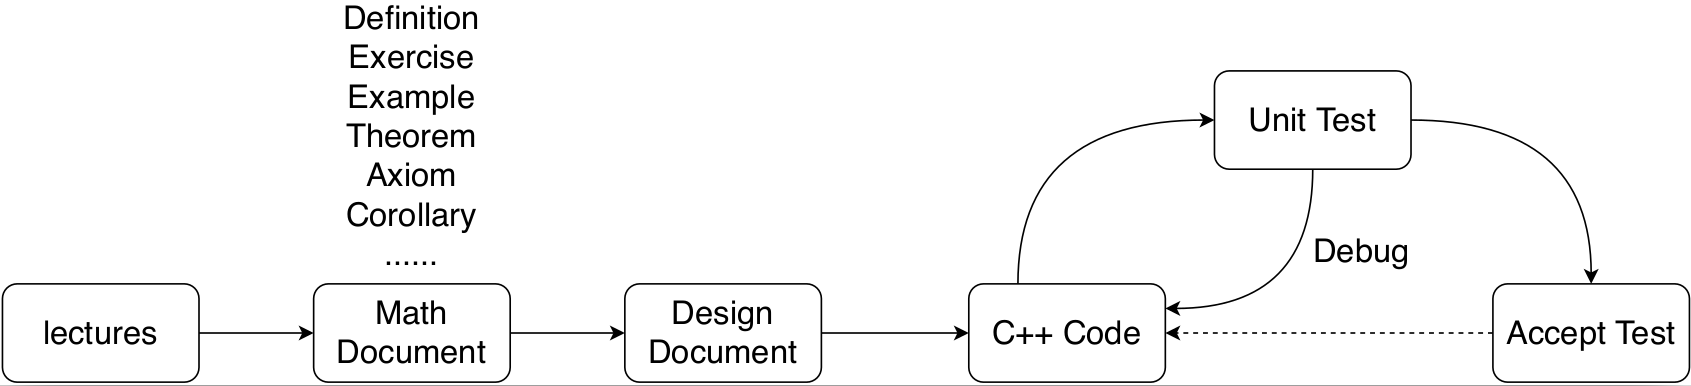
\includegraphics[width=0.4\textdwidth]{png/designPattern.png}
%   \caption{Design pattern}
%   \label{fig:designpattern}
% \end{figure}
\begin{center}
  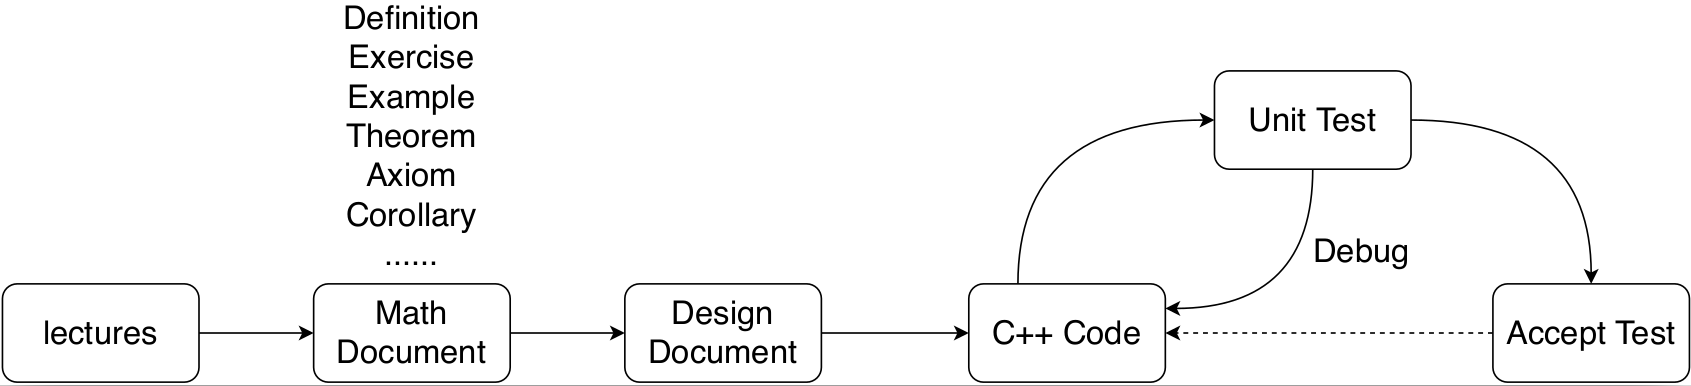
\includegraphics[width=0.45\textwidth]
     {png/designPattern.png}
\end{center}
\begin{thm}[The fundamental theorem of linear algebra]
  If $V$ is finite dimensional and $T\in {\cal L}(V,W),$
  then range $T$ is a finite-dimensional subspace of $W$
  and
  \begin{equation}
    \label{eq:1}
    \dim V= \dim {\cal N}( T)+ \dim {\cal R}(T).
  \end{equation}
\end{thm}

\begin{coro}
  For a matrix $A:\mathbb{R}^m\rightarrow\mathbb{R}^n$,
  \begin{align}
    \mathbb{R}^n&={\cal R}(A)\oplus {\cal N}(A^T),\label{eq:matrix}\\
    \mathbb{R}^m&={\cal R}(A^T)\oplus {\cal N}(A).
  \end{align}
  where ${\cal R}(A)\perp {\cal N}(A^T)$ and
  ${\cal R}(A^T)\perp {\cal N}(A)$.
\end{coro}

\begin{proof}
  For $\forall \mathbf{v}\in \{\mathbf{v}\in\mathbb{R}^m
  \vert A\mathbf{v}\in {\cal N}(A^T)\},$
  we have
  \begin{equation*}
    \grb{A\mathbf{v},\mathbf{v}}
    =\grb{\mathbf{v},A^T\mathbf{v}}=0,
  \end{equation*}
  which implies $\mathbf{v}=\mathbf{0}$.
  Thus ${\cal R}(A)\cap {\cal N}(A^T)=\{\mathbf{0}\}$
  and (\ref{eq:2}) follows from (\ref{eq:1}).
\end{proof}

%%% Local Variables:
%%% mode: latex
%%% TeX-master: "../notesNumericalSolution"
%%% End:



%\input{sec/introduction.tex}

\end{multicols}

\chapter{Geometric multigrid methods}
\label{cha:geom-mult-meth}

\begin{multicols}{2}
\setlength{\columnseprule}{0.2pt}  

Motivation of multigrids
\begin{itemize}
\item The convergence rates of classical iterative method
  depend on the grid spacing, or problem size.
  In contrast, convergence rates of multigrid methods does not.
\item  The complexity is $O(n)$.
\end{itemize}

From continuous contract to discrete contract.
Given the differential equation:

\paragraph{continuous contract}
\begin{enumerate}
\item [input:] the boundary conditions,

\item  [output:] the function in the domain.
\end{enumerate}
\paragraph{discrete contract}
\begin{enumerate}
\item [input:] the boundary conditions and the grid points

 \item [output:] the function in the grid points
\end{enumerate}


\begin{CJK*}{UTF8}{gkai}
  多重网格运用迭代法的思路,
  把难的问题分解成几个简单的问题.
  最重要的科研能力是把困难的问题变成简单的问题.
  各个简单的小问题之间形成图的关系$G=(V,E),
  E:V\times V\rightarrow \{0,1\}$.
\end{CJK*}
Two relations:
\begin{itemize}
\item " is a ": polymonphism,
\item " has a ": composition.
\end{itemize}
\section{Model problems}
\label{sec:model-problems}

On the unit 1D domain $x\in[0,1]$,
we numerically solve Poisson equation with homogeneous boundary condition
\begin{displaymath}
  -\Delta u = f, \quad u(0) = u(1) = 0.
\end{displaymath}
Discretize the domain with $n$ cells and locate the knowns $f_j$
and unknows $u_j$ at nodes $x_j= j/n = jh,j=0,1,...,n.$
We would like to approximate the second derivative of $u$
using the dicrete values at the nodes.
Using Taylor expansion, we have
\begin{equation}
  \label{eq:2}
  \frac{\partial ^2u}{\partial x^2}\vert_{jh}
  =\frac{u_{j+1}+u_{j-1}-2u_j}{h^2}+O(h^2).
\end{equation}


\begin{defn}
  The 1-D 2nd-order discrete Laplacian
  is a Toeplitz matrix $A\in \mathbb{R}^{(n-1)\times (n-1)}.$
  \begin{equation}\label{eq:discreteLaplacian}
    a_{ij}=
    \begin{cases}
      \frac{2}{h^2},\ &\textmd{if}\ i=j,\\
      -\frac{1}{h^2},\ &\textmd{if}\ \vert i-j\vert=1,\\
       0,\ &\textmd{otherwise}
    \end{cases}
  \end{equation}
\end{defn}

\begin{ntn}
  The linear system for 1D Possion equation:
  \begin{equation}\label{eq:linearSystem-1D}
    A\mathbf{u}=\mathbf{f},
  \end{equation}
where $f_j=h^2f(x_j).$
\end{ntn}

\begin{prop}
  \begin{equation}
    \frac{1}{h^2}(Au)_j-(\Delta u)\vert_{x_j}= O(h^2),
    \forall j=1,\ldots, n-1.
  \end{equation}
\end{prop}

\begin{prop}
  The eigenvalues $\lambda_k$ and eigenvectors $\mathbf{w}_k$
  of $A$ are
  \begin{equation}
    \lambda_k(A)= 4\sin^2\frac{k\pi}{2n},
  \end{equation}
  \begin{equation}
    \omega_{k,j}=\sin \frac{jk\pi}{n},
  \end{equation}
  where $j,k=1,2,...,n-1.$
\end{prop}

\begin{solution}
  Use the trigonmetric identity
  \begin{equation}
    \sin \alpha+\sin \beta = 2 \sin \frac{\alpha + \beta}{2}
    \cos \frac{\alpha - \beta}{2}
  \end{equation}
\end{solution}

\section{The residual equation}
% \section{Basic iterative methods}

% \label{sec:basic-iter-meth}
\begin{ntn}
  Let
  \begin{displaymath}
    A\mathbf{u}=\mathbf{f}
  \end{displaymath}
  denote a system of linear equation
  with a unique solution.
  We use $\mathbf{u}$ to denote
  the exact solution of this system
  and
  % $\tilde{\mathbf{u}}$
  $\mathbf{v}$ to denote
 a computed approximation to $\mathbf{u}$.
\end{ntn}

\begin{defn}
  The \emph{error} (or \emph{algebraic error})
  is given by
  \begin{displaymath}
    \mathbf{e}=\mathbf{u}-\mathbf{v}.
  \end{displaymath}
The \emph{residual} is given by
\begin{equation}
 \mathbf{r}=\mathbf{f}-A\mathbf{v}.
\end{equation}
Then
\begin{equation}
  A\mathbf{e}=r
\end{equation}
holds and it is called the residual equation.
\end{defn}

\begin{rem}
  The residual is simply the amount by which
  the approximation $\mathbf{v}$ fails to satisfy the original problem
  $\mathbf{r}=\mathbf{f}-A\mathbf{v}$.

  As one advantage,
  the residual equation lets us focus on homogenuous Dirichlet
  condition WLOG.

  For inexact arithmetic,
  a small residual does not imply a small error.
\end{rem}

\begin{defn}
  The condition number of a matrix $A$ is \emph{cond}
  $(A)=\Vert A\Vert_2\Vert A^{-1}\Vert_2.$
  It indicates how well the residual measures the error.
  \begin{equation}
    \begin{aligned}
      \Vert A\Vert_2 &= \sup_{\mathbf{x}\neq 0}
      \frac{\Vert A\mathbf{x}\Vert_2}{\Vert \mathbf{x}\Vert_2}\\
      &=\sup_{\mathbf{x}\neq 0}
      \sqrt{\frac{(
          A\mathbf{x},A\mathbf{x})}{(\mathbf{x},\mathbf{x})}}\\
      &=\sup_{\mathbf{x}\neq 0}
      \sqrt{\frac{(
          \mathbf{x},A^TA\mathbf{x})}{(\mathbf{x},\mathbf{x})}}\\
      &=\sqrt{\lambda_{\max}(A^TA)}
    \end{aligned}
  \end{equation}
  Since $A$ is symmetric,
  $\Vert A\Vert_2=\lambda_{\max}(A)$.
  $\Vert A^{-1}\Vert_2=\lambda_{\max}(A^{-1})=\lambda^{-1}_{\min}(A)$.
\end{defn}

% \begin{lem}
%   The \emph{residual equation}
%   \begin{displaymath}
%     A\mathbf{e}=\emph{r}.
%   \end{displaymath}
% \end{lem}

\begin{thm}
  \begin{equation}
    \frac{1}{cond(A)}\frac{\Vert\mathbf{r}\Vert_2}{\Vert
      \mathbf{f}\Vert_2}
    \leq \frac{\Vert\mathbf{e}\Vert_2}{\Vert
      \mathbf{u}\Vert_2}
    \leq cond(A)\frac{\Vert\mathbf{r}\Vert_2}{\Vert
      \mathbf{f}\Vert_2}
  \end{equation}
\end{thm}
\begin{proof}
  \begin{equation}
    \begin{aligned}
       \frac{1}{cond(A)}\frac{\Vert\mathbf{r}\Vert_2}{\Vert
         \mathbf{f}\Vert_2}
       &=  \frac{1}{\Vert A\Vert_2\Vert A^{-1}\Vert_2}
       \frac{\Vert A\mathbf{e}\Vert_2}{\Vert
         \mathbf{f}\Vert_2}\\
       &\leq  \frac{\Vert A\Vert_2\Vert \mathbf{e}\Vert_2}
       {\Vert A\Vert_2\Vert A^{-1}\mathbf{f}\Vert_2}
       =\frac{\Vert\mathbf{e}\Vert_2}{\Vert
         \mathbf{u}\Vert_2}\\
       &\leq \frac{\Vert A\Vert_2\Vert A^{-1}\mathbf{r}\Vert_2}
       {\Vert A\Vert_2\Vert
         \mathbf{u}\Vert_2}=
       cond(A)\frac{\Vert\mathbf{r}\Vert_2}{\Vert
      \mathbf{f}\Vert_2}.
    \end{aligned}
  \end{equation}
\end{proof}

\section{Fourier modes}

\begin{ntn}
  Hereafter $\Omega^h$ denote both the uniform grid with $n$ intervals
  and the corresponding vector space.

  Wavelength refers to the distance of one sinusoidal period.

  The wavenumber $k$ is the number of half sinusoidal waves in the domain.
\end{ntn}

\begin{prop}
  The $k$th Fourier mode $\omega_{k,j}=\sin(x_jk\pi)$
  has wavelength $L_{\omega}=\frac{2}{k}.$
\end{prop}

\begin{proof}
  $\sin(x_jk\pi)=-\sin(x_j+\frac{L}{2})k\pi$
  implies $x_j k\pi=(x_j+\frac{L}{2})k\pi-\pi$.
  Hence $L_{\omega}=\frac{2}{k}.$
\end{proof}

\begin{defn}
  On $\Omega^h,$
  the Fourier modes with wavenumbers $k\in [1,n/2)$
  are called \emph{low-frenquency}(LF) or \emph{smooth} modes,
  those with $k\in [n/2,n)$ \emph{high-frenquency}(HF) or \emph{oscillatory}
  modes.
\end{defn}


\section{Weighted Jacobi}

\label{sec:weighted-jacobi}

The scalar fixed-point iteration converts the problem of finding
a root of $f(x)=0$ to the problem of finding a fixed point of $g(x)=x$
where $f(x)=c(g(x)-x),c\neq 0.$

Decompose $A$ as $A=D+L+U.$
Jacobi iteration has $M=D,N=-(L+U),T=-D^{-1}(L+U).$
Here $T=I-\frac{1}{2}A$, $\rho(T)=1-2\sin^2\frac{\pi}{2n}$.
as $h\rightarrow 0,\rho(T)\rightarrow 1$,
and Jacobi converges slowly.

Consider a generalization of the Jacobi iteration.

\begin{defn}
The weighted Jacobi is given by the following.
%\begin{equation}
  \begin{align}
    \mathbf{u}^*&=-D^{-1}(L+U)\emph{u}^{(\ell)}+D^{-1}\emph{f},\\
    \mathbf{u}^{(\ell +1)}&=(1-\omega)\mathbf{u}^{(\ell)}+
                            \omega\mathbf{u}^*.
  \end{align}
%\end{equation}
  Setting $\omega=1$ yields Jacobi.
\end{defn}

\begin{prop}
  The weighted Jacobi has the iteration matrix
  \begin{equation}
    T_{\omega}=(1-\omega)I-\omega D^{-1}(L+U)=I-\frac{\omega}{2}A,
  \end{equation}
  whose eigenvectors are the same as those of $A$,
  with the corresponding eigenvalues as
  \begin{equation}
    \lambda_k(T_{\omega})=1-2\omega\sin^2\frac{k\pi}{2n},
  \end{equation}
  where $k = 1,2,\ldots,n-1$.
\end{prop}

Write $\mathbf{e}^{(0)}=\sum_kc_k\mathbf{w}_k$,
then
\begin{equation}
  \mathbf{e}^{(\ell)}=T^{\ell}_{\omega}\mathbf{e}^{(0)}=
  \sum_kc_k\lambda^{\ell}_k(T_{\omega})\mathbf{w}_k.
\end{equation}
No value of $\omega$ will reduce the smooth components of the error
effectively.
\begin{equation}
  \lambda_1(T_{\omega})=1-2\omega\sin^2\frac{\pi}{2n}
  \approx 1-\frac{\omega\pi^2h^2}{2}.
\end{equation}

\begin{rem}
  Having accepted that no value of $\omega$ damps the smooth
  components satisfactorily,
  we ask what value of $\omega$ provides the best damping of
  the oscillatory modes.
\end{rem}

\begin{defn}
  The smoothing factor $\mu$ is the smallest factor by
  which the HF modes are damped per iteration.
  An iterative method is said to have the smoothing property
  if $\mu$ is small and independent of the grid size.
\end{defn}

\begin{exm}
  For weighted Jacobi, this leads to an optimization problem
  \begin{equation}
    \mu =\min_{\omega\in[0,1]}\max_{k\in[n/2,n)}\lambda_k(T_{\omega})
    \Rightarrow \omega=\frac{2}{3}.
  \end{equation}
  And the smoothing factor is $\frac{1}{3}$.
\end{exm}


\section{Two-grid correction}

\label{sec:two-grid-correction}

\begin{prop}
  \label{prop:twoGridModes}
  The $k$-th mode on $\Omega^h$ becomes the $k$th mode on $\Omega^{2h}$:
  \begin{equation}
    \omega^h_{k,2j}=\omega^{2h}_{k,j}.
  \end{equation}
  However,
  the LF modes $k\in [\frac{n}{4},\frac{n}{2})$ of $\Omega^h$ will
  become HF modes on $\Omega^{2h}$.
\end{prop}

\begin{proof}
  \begin{equation}
    \omega^h_{k,2j}=\sin\frac{2jk\pi}{n}=\sin\frac{jk\pi}{n/2}
    =\omega^{2h}_{k,j},
  \end{equation}
  where $k\in[1,n/2)$.
  The mode with $k\in [\frac{n}{4},\frac{n}{2})$
  are HF on $\Omega^{2h}$ by definition since the
  highest wavenumber is $\frac{n}{2}$ on $\Omega^{2h}$.
\end{proof}

\begin{defn}
  The restriction operator $I^{2h}_h:\mathbb{R}^{n-1}\rightarrow
  \mathbb{R}^{n/2-1}$ maps a vector on the fine grid $\Omega^h$
  to its counterpart on the coarse grid $\Omega^{2h}:$
  \begin{equation}
    I^{2h}_hv^h=v^{2h}.
  \end{equation}
\end{defn}

\begin{exm}
  A common restriction operator is the full-weighting operator
\begin{equation}
  v^{2h}_j=\frac{1}{4}(v^h_{2j-1}+2v^h_{2j}+v^h_{2j+1}),
\end{equation}
where $j=1,2,...,\frac{n}{2}-1$.
For $n=8,$
   \begin{equation}
     I^{2h}_{h}=\frac{1}{4}
     \begin{bmatrix}
       1 & 2& 1 & & & &\\
         & & 1  &2&1& &\\
        & &     & & 1&2&1\\
     \end{bmatrix}.
   \end{equation}
\end{exm}

\begin{defn}
  The prolongation or interpolation operator
  $I^h_{2h}:\mathbb{R}^{n/2-1}\rightarrow \mathbb{R}^{n-1}$
  maps a vector on the coarse grid $\Omega^{2h}$
  to its countrtpart on the fine grid $\Omega^h$:
  \begin{equation}
    I^h_{2h}v^{2h}=v^{h}.
  \end{equation}
\end{defn}


\begin{exm}\label{exm:linear}
   A common prolongation is the linear interpolation operator
  \begin{equation}
    \begin{aligned}
      v^h_{2j}&=v^{2h}_j,\\
      v^{h}_{2j+1}&=\frac{1}{2}(v^{2h}_j+v^{2h}_{j+1}).
    \end{aligned}
  \end{equation}
   For $n=8$
   \begin{equation}
     I^h_{2h}=\frac{1}{2}
     \begin{bmatrix}
       1 & &\\
       2& &\\
       1&1&  \\
       & 2& \\
       &1&1\\
       & & 2\\
       & & 1\\
     \end{bmatrix}.
   \end{equation}

  \end{exm}

  \begin{rem}
    The key idea is that the weighted Jacobi with $\omega
    =\frac{2}{3}$
    damps HF modes effectively,
    we can exploit this on a series of successively coarsened grides
    to eliminite HF modes.
  \end{rem}

  \begin{defn}
    For $Au=f,$
    the two grid correction scheme
    \begin{equation}
      \mathbf{v}^h\leftarrow  MG(\mathbf{v}^h,\mathbf{f}^h,\nu_1,\nu_2)
    \end{equation}
    consists of the following steps.
    
    1) Relax $A^h\mathbf{u}^h=\mathbf{f}^h$ $\nu_1$
    times on $\Omega^h$ with initial guess
    $\mathbf{v}^h:\mathbf{v}^h\leftarrow
    T_{\omega}^{\nu_1}\mathbf{v}^h +\mathbf{c}$,

    2) compute the fine-grid residual $\mathbf{r}^h=\mathbf{f}^h-
    A^h\mathbf{v}^h$ and restric it to the coarse grid by
    $\mathbf{r^{2h}}=I^{2h}_h\mathbf{r}^h$,

    3) slove $A^{2h}\mathbf{e}^{2h}=\mathbf{r}^{2h}$
    on $\Omega^{2h}: \mathbf{e}^{2h}\leftarrow
    (A^{2h})^{-1}\mathbf{r}^{2h},$
    
    4) interpolate the coarse-grid error to the fine grid by
    $\mathbf{e}^h=I^hh_{2h}\mathbf{e}^{2h}$
    and correct the fine-grid approximation:
    $\mathbf{v}^h\leftarrow \mathbf{v}^h+I^h_{2h}\mathbf{e}^{2h}$,

    5) relax $A^h\mathbf{u}^h=\mathbf{f}^{h}$ $\nu_2$ times
    on $\Omega^h$ with initial guess
    $\mathbf{v}^h:\mathbf{v}^h\leftarrow
    T_{\omega}^{\nu_2}\mathbf{v}^h
    +\mathbf{c}.$
  \end{defn}
  
  \begin{prop}
 Let TG denote the iteration matrix of the two-grid correction schme.
Then
\begin{equation}
\label{eq:TG}
  TG=T^{\nu_2}_{w}[I-I^h_{2h}(A^{2h})^{-1}I^{2h}_hA^h]T^{\nu_1}_{\omega}
\end{equation}
  \end{prop}

  \begin{proof}
    By definition,
the two-grid correction scheme replaces
the initial guess with
\begin{equation}
  \mathbf{v}^h\leftarrow  
T^{\nu_2}_{\omega}\mathbf{v}^h
+\mathbf{c}+T^{\nu_2}_{\omega}I^h_{2h}(A^{2h})^{-1}I^{2h}_h
[\mathbf{f}^h-A^h(T_{\omega}^{\nu_1}\mathbf{v}^h+\mathbf{c})],
\end{equation}
which also holds for the exact solution $\mathbf{u}^h$.
Subtracting the two equations yields (\ref{eq:TG}).
  \end{proof}

\section{Spectral and algebraic pictures}
\label{sec:spectr-algebr-pict}

\begin{rem}
  Our objective is to show that $\rho(TG)\approx 0.1$
for $\nu_1=2,\nu_2=0$.
For this purpose, 
we need to examine the intergrid transfer operators.
\end{rem}
\begin{defn}
  $\mathbf{w}^h_k(k\in [1,n/2))$ and $\mathbf{w}^h_{k'}(k'=n-k)$
are called complementary modes on $\Omega^h$. 
\end{defn}

\begin{prop}
  \label{prop:comolementary}
  For a pair of complementary modes on $\Omega^h$,
we have
\begin{equation}
  \omega_{k',j}^h=(-1)^{j+1}\omega^h_{k,j}.
\end{equation}
\end{prop}

\begin{proof}
  \begin{equation}
    \begin{aligned}
      w^h_{k',j}&=\sin \frac{(n-k)j\pi}{n}\\
&=\sin(j\pi-\frac{jk\pi}{n})
      =(-1)^{j+1}\omega^h_{k,j}.
    \end{aligned}
\end{equation}
\end{proof}


\begin{lem}
  The action of the full-weighting operator on a pair of complementary
modes is
\begin{align}
  I^{2h}_h\mathbf{w}^h_k&=\cos^2\frac{k\pi}{2n}\mathbf{w}^{2h}_k
=c_k\mathbf{w}_k^{2h},\\
  I^{2h}_h\mathbf{w}^h_{k'}&=-\sin^2\frac{k\pi}{2n}\mathbf{w}^{2h}_k
=-s_k\mathbf{w}_k^{2h},
\end{align}
where $k\in [1,n/2),k'=n-k.$
In addition, $ I^{2h}_h\mathbf{w}^h_{n/2}=0$.
\end{lem}

\begin{proof}
  For the LF mode,
  \begin{equation*}
    \begin{aligned}
      (I^{2h}_h\mathbf{w}^h_{k})_{,j}&=
      \frac{1}{4}\sin\frac{(j-1)k\pi}{n}
      +\frac{1}{2}\sin\frac{jk\pi}{n}
      +\frac{1}{4}\sin\frac{(j+1)k\pi}{n}\\
     & =\cos^2\frac{k\pi}{2n}\sin\frac{jk\pi}{n}
      =\cos^2\frac{k\pi}{2n}\mathbf{w}^{2h}_{k,j}
    \end{aligned}
  \end{equation*}
  where the last step follows Proposition \ref{sec:two-grid-correction}.
  As for the HF mode,
  follow the same procedure,
  we have
    \begin{equation*}
    \begin{aligned}
      (I^{2h}_h\mathbf{w}^h_{k})_{,j}&=
      -\sin^2\frac{k\pi}{2n}\sin\frac{jk\pi}{n}
      =-\sin^2\frac{k\pi}{2n}\mathbf{w}^{2h}_{k,j}
    \end{aligned}
  \end{equation*}
\end{proof}

\begin{rem}
  The full-weighting operator thus maps a pair of complementary modes
  to a multiple of the mode on the coarse grid.
\end{rem}

\begin{lem}
  The action of the linear interpolation operator on $\Omega^{2h}$ is
  \begin{equation}
    I^h_{2h}\mathbf{w}_k^{2h}=c_k\mathbf{w}^h_h-s_k\mathbf{w}^h_k,
  \end{equation}
where $k\in [1,n/2),k'=n-k.$
\end{lem}

\begin{proof}
  It follows by Proposition \ref{prop:comolementary} and
  trignometric identities that
  \begin{equation*}
    \begin{aligned}
      (c_k\mathbf{w}^h_h-s_k\mathbf{w}^h_k)_{,j}
      &=\left(\cos^2\frac{k\pi}{2n}+(-1)^j\sin^2\frac{k\pi}{2n}\right)
      \mathbf{w}^h_{k,j} \\
      &=
      \begin{cases}
        \mathbf{w}^h_{k,j},&j\textmd{ is even,}\\
        \cos\frac{k\pi}{n}\mathbf{w}^h_{k,j},&j\textmd{ is odd.}
      \end{cases}
    \end{aligned}
  \end{equation*}
   Example \ref{exm:linear} yields that
  \begin{equation*}
    \begin{aligned}
      &(I^h_{2h}\mathbf{w}^{2h}_k)_j\\
      =&
    \begin{cases}
      \mathbf{w}^h_k,&j\textmd{ is even,}\\
      \frac{1}{2}\sin\frac{k\pi(j-1)/2}{n/2}
      + \frac{1}{2}\sin\frac{k\pi(j-1)/2}{n/2},&j\textmd{ is odd.}
    \end{cases}
    \end{aligned}
  \end{equation*}
\end{proof}
\begin{rem}
  The range of the interpolation operator contains
  both smooth and oscillatory modes.
  In other words, it excites oscillatory modes
  on the fine grid.
  However, $if k\ll n,$
  the amplitudes of these HF modes $s_k \sim O(\frac{k^2}{n^2})$.
\end{rem}

\begin{thm}
  The two-grid correction operator is invarianat on the subspace
  $W^h_k=\textmd{span}\{\mathbf{w}^h_{k},\mathbf{w}^h_{k'}\} $.
  \begin{equation}
    \begin{aligned}
      TG
      \begin{bmatrix}
        \mathbf{w}_k\\
        \mathbf{w}_{k'}
      \end{bmatrix}
      &=
      \begin{bmatrix}
        \lambda_k^{\nu_1+\nu_2}s_k&\lambda_k^{\nu_1}\lambda_{k'}^{\nu_2}s_k\\
        \lambda_{k'}^{\nu_1}\lambda_{k}^{\nu_2}c_k&\lambda_{k'}^{\nu_1+\nu_2}c_k
      \end{bmatrix}
      \begin{bmatrix}
        \mathbf{w}_k\\
        \mathbf{w}_{k'}
      \end{bmatrix}\\
      &=
      \begin{bmatrix}
        c_1 & c_2\\
        c_3& c_4
      \end{bmatrix}
      \begin{bmatrix}
        \mathbf{w}_k\\
        \mathbf{w}_{k'}
      \end{bmatrix}
    \end{aligned}
  \end{equation}
  where $\lambda_k$ is the eigenvalue of $T_{\omega}$.
\end{thm}

\begin{proof}
  Consider the case of $\nu_1=\nu_2=0$.
  \begin{subequations}
    \begin{align}
      &A^h\mathbf{w}^h_k=4s_k\mathbf{w}^h_k\\
      \Rightarrow
      &I^{2h}_hA^h\mathbf{w}^h_k=16c_ks_k\mathbf{w}^{2h}_k
      \label{eq:residualScaled}\\
      \Rightarrow &(A^{2h})^{-1} I^{2h}_hA^h\mathbf{w}^h_k=
                    \frac{16c_ks_k}{4\sin^2\frac{k\pi}{n/2}}\mathbf{w}^{2h}_k=
                    \mathbf{w}^{2h}_k\\
      \Rightarrow &-I^h_{2h}(A^{2h})^{-1} I^{2h}_hA^h\mathbf{w}^h_k=
                    -c_k\mathbf{w}^h_k+s_k\mathbf{w}^{h}_{k'}\\
       \Rightarrow &[I-I^h_{2h}(A^{2h})^{-1} I^{2h}_hA^h]\mathbf{w}^h_k=
                    s_k\mathbf{w}^h_k+s_k\mathbf{w}^{h}_{k'},\label{eq:01}
    \end{align}
  \end{subequations}
  where the additional factor of 4 comes from the fact that
  the residual is scaled by $h^2$.
  Similarly,  \begin{subequations}
    \begin{align}
      &A^h\mathbf{w}^h_{k'}=4s_{k'}\mathbf{w}^h_{k'}=4c_k\mathbf{w}^h_{k'}
      \\
      \Rightarrow
      &I^{2h}_hA^h\mathbf{w}^h_{k'}=-16c_ks_k\mathbf{w}^{2h}_k
      \label{eq:residualScaled}\\
      \Rightarrow &(A^{2h})^{-1} I^{2h}_hA^h\mathbf{w}^h_{k'}=
                  -  \frac{16c_ks_k}{4\sin^2\frac{k\pi}{n/2}}\mathbf{w}^{2h}_k=
                    -\mathbf{w}^{2h}_k\\
      \Rightarrow &-I^h_{2h}(A^{2h})^{-1} I^{2h}_hA^h\mathbf{w}^h_{k'}=
                    c_k\mathbf{w}^h_k-s_k\mathbf{w}^{h}_{k'}\\
       \Rightarrow &[I-I^h_{2h}(A^{2h})^{-1} I^{2h}_hA^h]\mathbf{w}^h_{k'}=
                    c_k\mathbf{w}^h_k+c_k\mathbf{w}^{h}_{k'},\label{eq:02}
    \end{align}
  \end{subequations}
  Adding pre-smoothing incurs a scaling of $\lambda_k^{\nu_1}$
  for (\ref{eq:01}) and $\lambda^{\nu_1}_{k'}$ for (\ref{eq:02}).
  In contrast,
  adding postsmoothing incurs a scaling of $\lambda_k^{\nu_2}$
  for $\mathbf{w}_k^h$ and a scaling of $\lambda_{k'}^{\nu_2}$
  for $\mathbf{w}^h_{\omega}$.
\end{proof}

\begin{lem}
  The full-weighting operator and the linear-interpolation
  operator satisfy the variational properties
  \begin{subequations}
    \begin{align}
      I^h_{2h}=c(I^{2h}_h)^T, c\in \mathbb{R},\label{eq:variational}\\
      I^{2h}_hA^hI^h_{2h}=A^{2h}.\label{eq:galerkin}
    \end{align}
  \end{subequations}
(\ref{eq:galerkin}) is also called the Galerkin condition.
\end{lem}

\begin{prop}
  A basis for the range of the interpolation operator
  ${\cal R}(I^h_{2h})$ is given by its columns,
  hence $\dim {\cal R}(I^h_{2h})=\frac{n}{2}-1,{\cal N}(I^h_{2h})=0.$
\end{prop}

\begin{coro}
For the full-weighting operator,
\begin{equation}
  \dim {\cal R}(I^{2h}_h)=\frac{n}{2}-1,
  \dim {\cal N}(I^{2h}_h)=\frac{n}{2}.
\end{equation}
\end{coro}

\begin{proof}
 Follows form (\ref{eq:matrix}) and (\ref{eq:variational}).
\end{proof}

\begin{thm}
  The null space of the two-grid correction operator is the range of
  interpolation:
  \begin{equation}
    {\cal N}(TG)={\cal R}(I^h_{2h}).
  \end{equation}

\end{thm}




\section{Multigrid cycles}
\label{sec:multigrid-cycles}
\begin{defn}
  The \emph{V-cycle scheme} is an algorithm
  \begin{equation}
    \mathbf{v}^h\leftarrow V^h(\mathbf{v}^h,\mathbf{f}^h,\nu_1,\nu_2)
  \end{equation}
  with the following steps.
  
  1) Relax $\nu_1$ times on $A^h\mathbf{u}^h=\mathbf{f}^h$
  with a given initial guess $\mathbf{v}^h$,

  2) if $\Omega^h$ is the coarset grid,
  go to step 4), otherwise
  \begin{equation*}
    \begin{aligned}
      &\mathbf{f}^{2h}\leftarrow
        I^{2h}_h(\mathbf{f}^h-A\mathbf{v}^h),\\
        &\mathbf{v}^{2h}\leftarrow \mathbf{0},\\
        &\mathbf{v}^{2h}\leftarrow V^{2h}(\mathbf{v}^{2h},\mathbf{f}^{2h}),
    \end{aligned}
  \end{equation*}
  3) interpolate error back and correct the solution:
  $\mathbf{v}^h\leftarrow \mathbf{v}^h+I^h_{2h}\mathbf{v}^{2h}$,

  4) relax $\nu_2$ times on $A^h\mathbf{u}^h=\mathbf{f}^h$
  with the initial guess $\mathbf{v}^h$.
\end{defn}

\begin{defn}
  The \emph{Full Multigrid V-cycle} is an algorithm
  \begin{equation}
    \mathbf{v}^h\leftarrow FMG^h(\mathbf{f}^h,\nu_1,\nu_2)
  \end{equation}
  with the following steps.

  1) If $\Omega^h$ is the coarest grid,
  set $\mathbf{v}^h\leftarrow \mathbf{0}$ and go to step 3),
  otherwise
  \begin{equation*}
    \begin{aligned}
      &\mathbf{f}^{2h}\leftarrow I^{2h}_h\mathbf{f}^h,\\
      &\mathbf{v}^{2h}\leftarrow FMG^{2h}(\mathbf{f}^{2h},\nu_1,\nu_2),
    \end{aligned}
  \end{equation*}
  
  2) correct $ \mathbf{v}^h\leftarrow I^h_{2h}\mathbf{v}^{2h},$

  3)% perform a V-cycle with the initial guess
  use the initial guess
  $\mathbf{v}^h\leftarrow V^h(\mathbf{v}^h,\mathbf{f}^h,\nu_1,\nu_2)$
  to perform a V-cycle.
\end{defn}

\begin{rem}
  We can see that FMG is a variation of V-cycle
  preceded by a coarse-grid V-cycle designed to provide the
  best initial guess possible.
\end{rem}

\begin{exc}
  The difference in cost between FMG and a single V-cycle
  is the cost of all but the last V-cycle on $\Omega^h$
  in the FMG scheme.
  
\end{exc}

\section{The 5-point stencil in 2D}
\label{sec:5-point-stencil}
\begin{exm}
  Consider the Poisson problem on the unit square
  $0\leq x\leq 1,0\leq y\leq 1$
  and suppose we have Dirichlet boundary conditions.
  \begin{displaymath}
    \begin{cases}
      u_{xx}+u_{yy}=f(x,y)\\
      u\vert_{\partial \Omega}=g(x,y)
    \end{cases}
  \end{displaymath}
  where $\Omega=(0,1)\times (0,1).$
\end{exm}
By formula (\ref{eq:2}), we have
\begin{equation}
  \label{eq:2-D-laplacian}
    \frac{u_{i-1,j}-2u_{i,j}+u_{i+1,j}}{h^2}+
    \frac{u_{i,j-1}-2u_{i,j}+u_{i,j+1}}{h^2}
    =f_{i,j},
  \end{equation}
  where $u_{i,j}$ is an approximation to $u(x_i,x_j)$
  and $f_{i,j}=f(x_i,x_j).$
and then using the natural rowwise ordering for $A_{2D}$,
as in the figure bellow
\begin{center}
  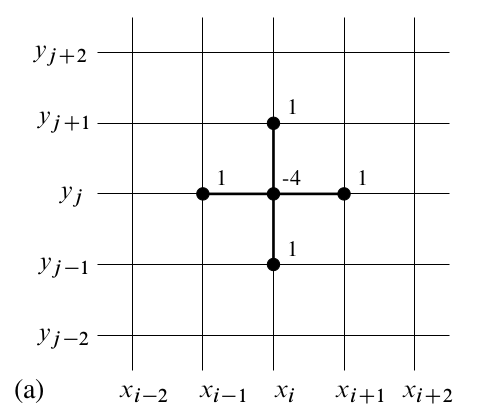
\includegraphics[width=0.4\textwidth]
  {png/rowwise.png}
\end{center}

\begin{rem}
  we have
  \begin{equation}
    \label{eq:2-Dpossion}
    A_{2D}U=-F.
  \end{equation}
\end{rem}


\begin{prop}
  \begin{equation}
    \label{eq:possionMatrix2D}
    AU_{m\times m}+U_{m\times m}A =  -F_{m\times m}
  \end{equation}
  where
  \begin{displaymath}
    U_{m\times m}=
    \begin{bmatrix}
      u_{11} & u_{12}& \ldots &u_{1m}\\
      u_{21} & u_{22} & \ldots & u_{2m} \\
      \vdots & \vdots &  & \vdots\\
      u_{m1} & u_{m2} & \ldots & u_{mm}
    \end{bmatrix},
    F=[f_{ij}]_{m\times m}.
  \end{displaymath}
\end{prop}

\begin{ntn}
  \begin{equation}
    \label{eq:A_2D}
    A_{2D}=AU_{m\times m}+U_{m\times m}A.
  \end{equation}
\end{ntn}

\begin{defn}
  For $A\in \mathbb{c}^{m\times n}, B\in \mathbb{C}^{p\times q}$,
  the kronecher product of $A$ and $B$ is
  \begin{equation}
    \label{eq:kronecher}
    A\otimes B=
    \begin{bmatrix}
      a_{11}B & a_{12}B &\ldots & a_{1n}B\\
      a_{21}B & a_{22}B & \ldots &a_{2n}B \\
      \vdots & \vdots & &\vdots \\
      a_{m1}B &a_{m2}B &\ldots & a_{mn}B
    \end{bmatrix}
  \end{equation}
\end{defn}

\begin{prop}
  The kronecher product satisfied
  \begin{enumerate}
  \item [a.] $A\otimes B\neq B\otimes A,$
    $\exists$ permutation matrices $P,Q$ s.t.
    $A\otimes B=P(B\otimes A)Q.$
  \item [b.] $A\otimes (B+C)=A\otimes B+ A\otimes C$,\\
    $(A+B)\otimes C=A\otimes B+A\otimes C.$ 
    \item [c.]$(kA)\otimes B=k(A\otimes B)=A\otimes (kB).$
    \item [d.]$(A\otimes B)\otimes C=A\otimes (B\otimes C).$
    \item [e.] $(A\otimes B)(C\otimes D)=(AC)\otimes (BD).$
    \item [f.] $(A\otimes B)^{-1}=A^{-1}\otimes B^{-1}.$
  \end{enumerate}
\end{prop}

\begin{exm}
  \begin{displaymath}
    \begin{bmatrix}
      1 & 2 \\
      3 & 4
    \end{bmatrix}\otimes
    \begin{bmatrix}
      0 & 5\\
      6 & 7
    \end{bmatrix}
=
\begin{bmatrix}
  0 & 5 & 0 & 10\\
  6 & 7 & 12 & 14 \\
  0 & 15 & 0 & 20 \\
  18 & 21 & 24 & 28 
\end{bmatrix}
  \end{displaymath}
\end{exm}

\begin{defn}
  For $X\in \mathbb{C}^{m\times n},
  Vec(X)$ is the colum vector obtained by
  stacking columns of $X$.
  \begin{equation}
    \textmd{Vec}(X)=
    \begin{bmatrix}
      X_1\\
      X_2\\
      \vdots\\
      X_n
    \end{bmatrix}
  \end{equation}
\end{defn}

\begin{CJK*}{UTF8}{gkai}
  \begin{rem}
    避免$u[i][j]$,数组是指针形式读内存慢,
    可以写一个class $u(i,j)$实现1-1对应,去掉指针的解析过程.
  \end{rem}
\end{CJK*}

\begin{thm}
  \label{thm:Vec}
  For $A\in \mathbb{R}^{m\times m},B\in \mathbb{R}^{n\times n}$,
  $X\in \mathbb{R}^{m\times n}$,
  we have
  \begin{subequations}
    \begin{align}
      & \textmd{Vec}(AX) \equiv (I_n\otimes A)\textmd{Vec}(X),
      \label{eq:AX}\\
      & \textmd{Vec}(XB) \equiv (B^T\otimes I_m)\textmd{Vec}(X).
        \label{eq:XB}
    \end{align}
  \end{subequations}
\end{thm}

\begin{proof}
   (\ref{eq:AX}) is a direct conclusion from
  \begin{displaymath}
      \begin{bmatrix}
     AX_1\\
      AX_2\\
      \vdots\\
      AX_n
    \end{bmatrix}
    =
    \begin{bmatrix}
      A & & & \\
      & A &  & \\
      & & \ddots & \\
      & & & A
    \end{bmatrix}
  \begin{bmatrix}
      X_1\\
      X_2\\
      \vdots\\
      X_n
    \end{bmatrix}.
  \end{displaymath}
  The number of $XB$ in $i$-th row and $j$-th column
  is in the $((j-1)m+i)$-th row of Vec$(XB)$,
  which is equal to $\sum_{k=1}^{n}x_{ik}b_{kj}$.
  \begin{displaymath}
    \begin{aligned}
    &(B^T\otimes I_m)=
    \begin{bmatrix}
      b_{11}I_m & b_{21}I_m &\ldots & b_{n1}I_m\\
      b_{12}I_n & b_{22}I_m & \ldots & b_{n2}I_m\\
      \ldots & \ldots & & \\
      b_{1n}I_m & b_{2n}I_m & \ldots & b_{nn}I_m
    \end{bmatrix}\\
      & =
      \begin{bmatrix}
        b_{11} & & & \ldots&b_{n1} & &\\
        &\ddots &  &\ldots & &\ddots & \\
        & & b_{11}& \ldots & & &b_{n1}\\
        \ddots &  & & &\ddots & & \\
         & b_{1j} &\ldots  & b_{kj}&\ldots & b_{nj}& \\
        &  & \ddots & & & & \ddots\\
                      b_{1n} & & & \ldots&b_{nn} & &\\
        &\ddots &  &\ldots & &\ddots & \\
        & & b_{1n}& \ldots & & &b_{nn}\\
      \end{bmatrix}
       \begin{matrix}
          \\
          \\
          \\
          \\
          _{-((j-1)m+i)\textmd{-th}}\\
          \\
          \\
          \\
          \\
        \end{matrix}
    \end{aligned}
  \end{displaymath}
  It follows that the number of $ (B^T\otimes I_m)$Vec($X$)
  in the $((j-1)m+i)$-th row is $\sum_{k=1}^nb_{kj}x_{ik}$.
\end{proof}

\begin{coro}
  $AXB=C$ iff $A$ and $B$ are both invertible.
\end{coro}

\begin{proof}
  \begin{displaymath}
    \begin{aligned}
      \textmd{Vec}(AXB)&=(I_n\otimes A)\textmd{Vec}(XB)\\
      &=(I_n\otimes A)(B^T\otimes I_m)\textmd{Vec}(X)\\
      &=(B^T\otimes A)\textmd{Vec}(X).
    \end{aligned}
  \end{displaymath}
  It follows from 
  \begin{displaymath}
    (B^T\otimes A)^{-1}=(B^{T})^{-1}\otimes A^{-1}
  \end{displaymath}
that $AXB=C$ iff $A$ and $B$ are both invertible.
\end{proof}


\subsection{Relation of $A_{2D}$ and $A$}
\label{sec:relation}

\begin{lem}
  Let $A$ be the 1-D second-order discrete Laplacian
  (\ref{eq:discreteLaplacian}), then
  \begin{equation}
  \textmd{Vec}(AU_{m\times m}+U_{m\times m}A)=
  (I_m\otimes A+ A\otimes I_m)\textmd{Vec}(U_{m\times m}).
\end{equation}
\end{lem}

\begin{proof}
  By Theorem \ref{thm:Vec}, we have
  \begin{equation}
    \textmd{Vec}(AU_{m\times m})=(I_m\otimes A)\textmd{Vec}(U_{m\times m}),
  \end{equation}
  and 
  \begin{equation}
  \textmd{Vec}(U_{m\times m}A)=
  ( A^T\otimes I_m)\textmd{Vec}(U_{m\times m})
  = ( A\otimes I_m)\textmd{Vec}(U_{m\times m}),
\end{equation}
where the second equality follows from the symmetry of $A$.
Adding these two equations gives the desired result.
\end{proof}

\begin{thm}
  With matric ordering,
  the linear system (\ref{eq:linearSystem-1D}) can be written as
  \begin{equation}
    \begin{cases}
      A_{2D}=I_m\otimes A+ A\otimes I_m\\
      \mathbf{U}=\textmd{Vec}(U_{m\times m})\\
      \mathbf{F}=\textmd{Vec}(F_{m\times m})
    \end{cases}
  \end{equation}
\end{thm}

\begin{thm}
  The eigen-pairs of $A_{2D}$ are
  \begin{equation}
    \lambda_{ij}=\lambda_i+\lambda_j,
    \mathbf{v}_{ij}=\textmd{Vec}(\mathbf{v}^i(\mathbf{v}^j)^T),
  \end{equation}
where $(\lambda_i,\lambda_j)$ are for 1-D.
\end{thm}

%%% Local Variables:
%%% mode: latex
%%% TeX-master: "../notesNumericalSolution"
%%% End:


\end{multicols}

\bibliographystyle{abbrvnat}
\setcitestyle{authoryear,open={[},close={]}}

\end{document}



%%% Local Variables: 
%%% mode: latex
%%% TeX-master: t
%%% End: 

% LocalWords:  FPN underflows denormalized FPNs matlab eps IEEE iff
% LocalWords:  cardinality significand quadratically bijection unary
%  LocalWords:  contractive bijective postcondition invertible arity
%  LocalWords:  subspaces surjective injective monomials additivity
%  LocalWords:  nullary Abelian abelian finitary eigenvectors adjoint
%  LocalWords:  eigenvector nullspace Hermitian unitarily multiset
%  LocalWords:  nonsingular nonconstant homomorphism homomorphisms
%  LocalWords:  isomorphically indeterminates subfield isomorphism
%  LocalWords:  nondefective diagonalizable contrapositive cofactor
%  LocalWords:  submatrix nilpotent positivity orthonormal extremum
%  LocalWords:  Jacobian nonsquare semidefinite nonnegative RHS LLS
%  LocalWords:  roundoff closedness
